\DAsection[域名找服务器，Nginx 分流，证书建立信任]{域名、反向代理与 SSL 证书}

\begin{frame}{8.1 A 记录与 CNAME 记录}{一个指向 IP，一个指向另一个主机名}
  \begin{DAtable*}{@{}p{22mm}p{38mm}p{57mm}@{}}
    \toprule
    类型 & 示例 & 适用 \\
    \midrule
    A & \DAfile{@ \(\rightarrow\) 203.0.113.10} & 根域名指向 IPv4 服务器 \\
    AAAA & \DAfile{@ \(\rightarrow\) IPv6} & 使用 IPv6 时 \\
    CNAME & \DAfile{www \(\rightarrow\) example.com} & 子域名别名或第三方服务 \\
    TXT & 验证字符串 & 域名验证、邮件安全、ACME DNS-01 \\
    \bottomrule
  \end{DAtable*}
  \begin{itemize}
    \item \DAfile{@} 通常代表根域名，\DAfile{www} 代表 \DAfile{www.example.com}。
    \item 修改记录后存在缓存与 TTL，不同递归 DNS 生效时间可能不同。
  \end{itemize}
  \DAsource{Cloudflare DNS Docs · Record examples}{https://developers.cloudflare.com/dns/zone-setups/reference/dns-quick-scan/}
\end{frame}

\begin{frame}[fragile]{8.2 用 dig 验证 DNS}{同时检查 Host Header 与站点匹配}
  \begin{lstlisting}[language=bash]
dig +short app.example.com
dig app.example.com A
nslookup app.example.com

curl -I http://203.0.113.10 \
  -H "Host: app.example.com"
  \end{lstlisting}
  \begin{itemize}
    \item \DAcmd{dig} 验证域名解析结果。
    \item 带 Host Header 访问 IP，可区分 DNS 问题与 Nginx 站点配置问题。
    \item 使用 CDN / 代理 DNS 时，查询结果通常指向代理节点。
  \end{itemize}
\end{frame}

\begin{frame}{8.3 一个域名如何承载前后端}{推荐同域 + 路径分流}
  \begin{DAtable}{@{}p{31mm}p{41mm}p{46mm}@{}}
    \toprule
    方案 & 示例 & 特点 \\
    \midrule
    同域路径 & \DAfile{app.example.com/} + \DAfile{/api} & Cookie、CORS 最简单，课程默认 \\
    不同子域 & \DAfile{app.example.com} + \DAfile{api.example.com} & 边界清晰，需要配置 CORS / Cookie \\
    业务端口 & \DAfile{example.com:8000} & 不适合作为正式用户入口 \\
    \bottomrule
  \end{DAtable}
  \vspace{1mm}
  {\small\textcolor{DARed}{\bfseries 统一入口：}用户只访问 443，应用真实端口留在内部。}
\end{frame}

\begin{frame}[fragile]{8.4 代理头传递外部请求信息}{协议、域名与客户端 IP}
  \begin{lstlisting}[language=bash]
proxy_set_header Host $host;
proxy_set_header X-Real-IP $remote_addr;
proxy_set_header X-Forwarded-For $proxy_add_x_forwarded_for;
proxy_set_header X-Forwarded-Proto $scheme;
  \end{lstlisting}
  \begin{itemize}
    \item 后端生成重定向 URL、记录审计日志时需要外部请求信息。
    \item FastAPI 位于可信代理后时使用 \DAcmd{--proxy-headers}。
    \item 只信任可信反向代理写入的 \DAfile{X-Forwarded-For}。
  \end{itemize}
  \DAsource{FastAPI Docs · Behind a Proxy}{https://fastapi.tiangolo.com/advanced/behind-a-proxy/}
\end{frame}

\begin{frame}[fragile]{8.5 WebSocket 与 SSE 代理配置}{AI 流式输出的超时与缓冲}
  \begin{lstlisting}[language=bash]
# WebSocket
proxy_http_version 1.1;
proxy_set_header Upgrade $http_upgrade;
proxy_set_header Connection "upgrade";

# Server-Sent Events / streaming
proxy_buffering off;
proxy_read_timeout 3600s;
  \end{lstlisting}
  \begin{itemize}
    \item 普通 JSON 接口可以使用默认缓冲；流式响应需要尽快向客户端转发。
    \item 超时过短会让长回答中途断开；过长也要配合连接与资源限制。
    \item 在浏览器 Network 中确认数据持续到达。
  \end{itemize}
\end{frame}

\begin{frame}{8.6 Let's Encrypt / ACME 自动签发}{验证域名控制权并定期续期}
  \begin{columns}[T]
    \begin{column}{0.44\textwidth}
      \begin{enumerate}
        \item ACME Client 请求验证挑战。
        \item 通过 HTTP 文件或 DNS 记录证明控制域名。
        \item CA 从网络侧验证挑战。
        \item 生成 CSR 并签发证书。
        \item 客户端自动安装并定期续期。
      \end{enumerate}
    \end{column}
    \begin{column}{0.52\textwidth}
      \centering
      \DAframed{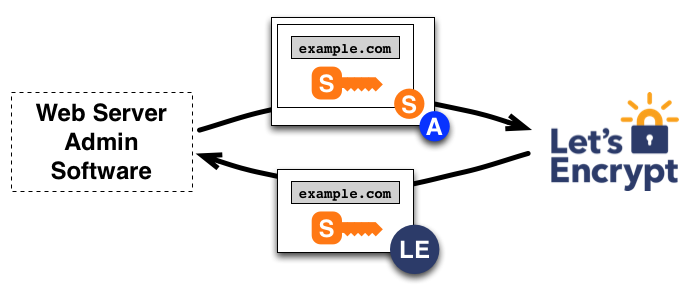
\includegraphics[width=65mm]{assets/official/letsencrypt-certificate.png}}
    \end{column}
  \end{columns}
  \DAsource{Let's Encrypt · How It Works}{https://letsencrypt.org/how-it-works/}
\end{frame}

\begin{frame}{8.7 HTTP-01 与 DNS-01 怎么选}{课堂单域名优先 HTTP-01}
  \begin{DAtable}{@{}p{25mm}p{44mm}p{51mm}@{}}
    \toprule
    验证方式 & 要求 & 适用 \\
    \midrule
    HTTP-01 & 域名已指向服务器，80 端口可访问 & 单域名、普通网站，配置简单 \\
    DNS-01 & 能通过 DNS 添加 TXT 记录 / API & 泛域名证书、80 不可达、集中证书管理 \\
    \bottomrule
  \end{DAtable}
  \begin{itemize}
    \item HTTP-01 申请失败先查 DNS、80 端口、防火墙和站点匹配。
    \item DNS API Token 使用最小权限，并像生产密钥一样保护。
  \end{itemize}
\end{frame}

\begin{frame}{8.8 宝塔申请与部署 SSL}{站点设置中完成申请、安装与续签}
  \begin{columns}[T]
    \begin{column}{0.50\textwidth}
      \centering
      \DAframed{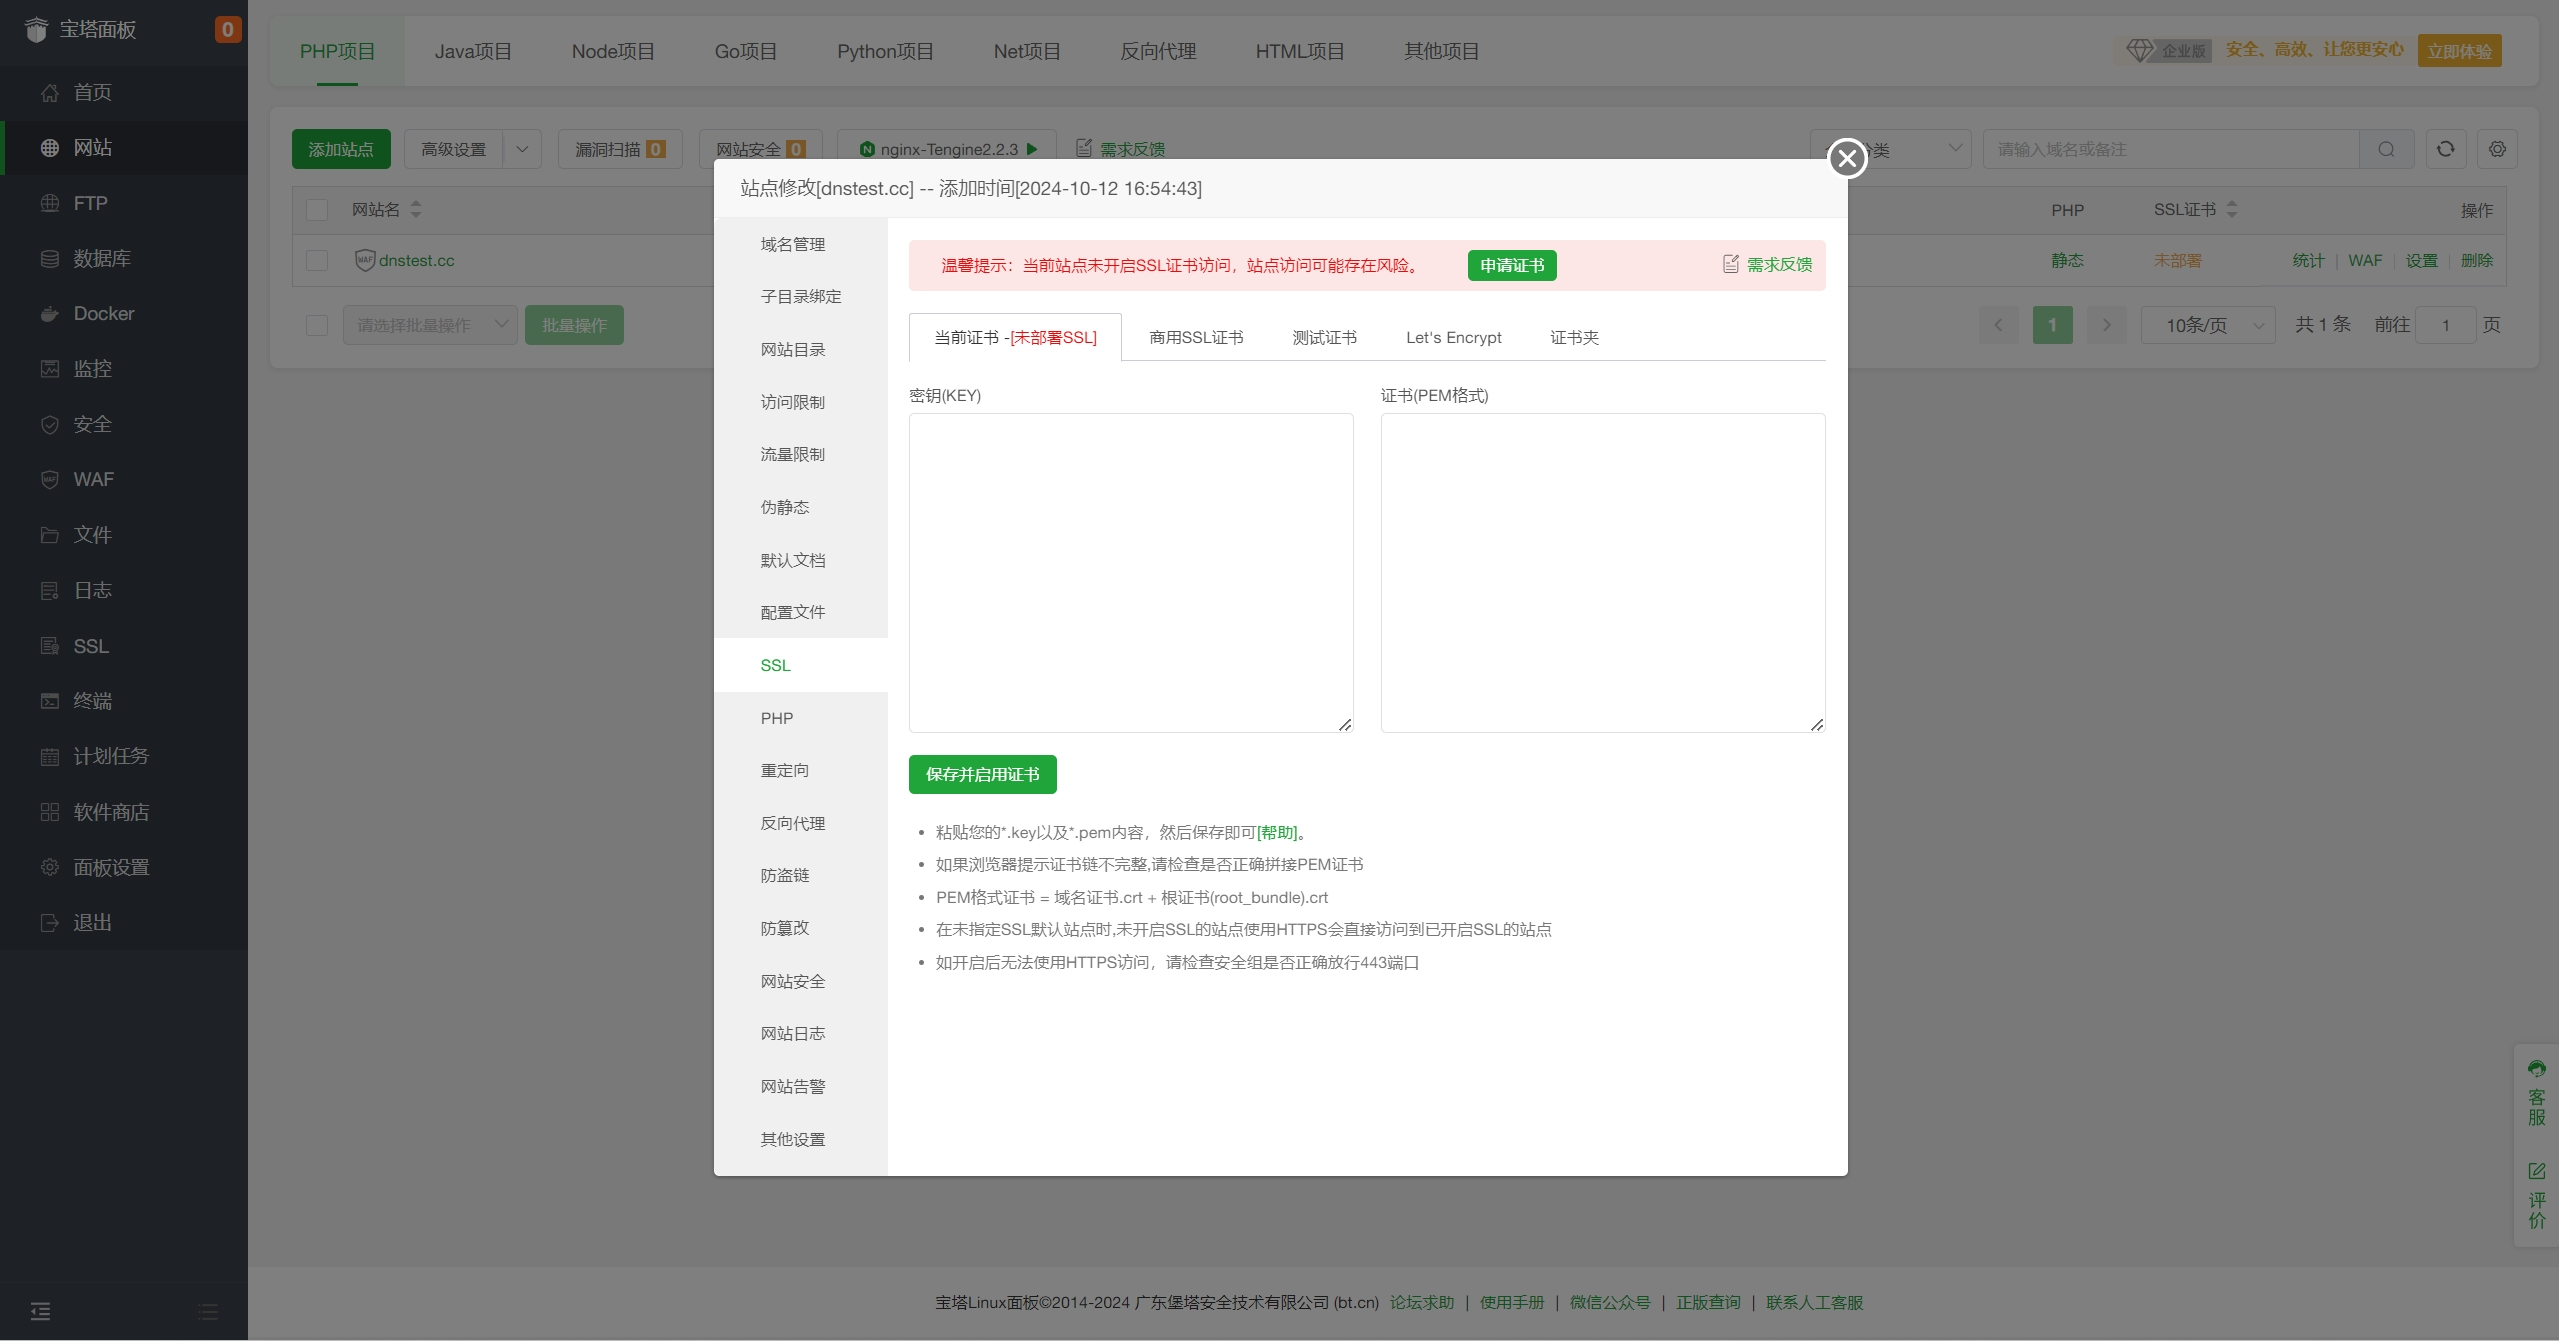
\includegraphics[height=39mm,trim=700 100 700 100,clip]{assets/official/bt-ssl.jpg}}
    \end{column}
    \begin{column}{0.46\textwidth}
      \begin{itemize}
        \item 域名先正确解析到服务器。
        \item 进入站点 SSL 页面申请。
        \item 可选免费证书或上传已有证书。
        \item 开启强制 HTTPS 与到期提醒。
      \end{itemize}
    \end{column}
  \end{columns}
  \DAsource{宝塔官方文档 · 部署 SSL 证书}{https://docs.bt.cn/getting-started/deploy-ssl}
\end{frame}

\begin{frame}[fragile]{8.9 HTTP 跳转 HTTPS}{80 端口保留验证与重定向}
  \begin{lstlisting}[language=bash]
server {
    listen 80;
    server_name app.example.com;

    location /.well-known/acme-challenge/ {
        root /www/server/panel/vhost/certbot;
    }

    location / {
        return 301 https://$host$request_uri;
    }
}
  \end{lstlisting}
  \begin{itemize}
    \item 宝塔通常会自动生成对应配置，不必手写路径。
    \item 强制 HTTPS 后，前端 API、图片、字体和 WebSocket 都应使用安全协议。
  \end{itemize}
\end{frame}

\begin{frame}{8.10 Mixed Content 排错}{HTTPS 页面中的 HTTP 请求会被拦截}
  \begin{alertblock}{典型错误}
    页面是 \DAfile{https://app.example.com}，前端仍请求 \DAfile{http://203.0.113.10:8000/api}。
  \end{alertblock}
  \begin{itemize}
    \item 浏览器会阻止不安全的 Fetch、XHR、Script、Stylesheet 等请求。
    \item 让 API、脚本、图片与 WebSocket 全部使用安全协议。
    \item 使用相对地址 \DAfile{/api}，可同时避免协议、域名与环境差异。
  \end{itemize}
  \DAsource{MDN · Mixed content}{https://developer.mozilla.org/en-US/docs/Web/Security/Defenses/Mixed_content}
\end{frame}

\begin{frame}{8.11 CORS 配置}{浏览器对跨 Origin 请求的约束}
  \begin{DAtable*}{@{}p{35mm}p{80mm}@{}}
    \toprule
    场景 & 处理 \\
    \midrule
    同域 \DAfile{/api} & 同源请求，配置最简 \\
    \DAfile{app.example.com} \(\rightarrow\) \DAfile{api.example.com} & 后端明确允许前端 Origin \\
    带 Cookie / Authorization & 不能用任意 \DAfile{*}；需精确 Origin 与 Credentials 配置 \\
    Postman / curl 能通，浏览器不通 & 优先检查 CORS 与 Preflight \\
    \bottomrule
  \end{DAtable*}
  \DAtagline{安全边界}{CORS 不能替代后端鉴权；攻击者可以不用浏览器直接请求 API}
\end{frame}

\begin{frame}[fragile]{8.12 上线后验证域名与证书}{检查跳转、证书、接口和安全头}
  \begin{lstlisting}[language=bash]
curl -I http://app.example.com
curl -I https://app.example.com
curl -i https://app.example.com/api/health

openssl s_client \
  -connect app.example.com:443 \
  -servername app.example.com </dev/null 2>/dev/null |
openssl x509 -noout -subject -issuer -dates
  \end{lstlisting}
  \begin{itemize}
    \item HTTP 应跳转 HTTPS；证书域名与有效期正确；API 返回预期 JSON。
    \item 浏览器控制台检查 Mixed Content、CORS、证书链与资源 404。
  \end{itemize}
\end{frame}

\begin{frame}{8.13 证书续签与 HSTS}{自动续签、到期提醒与安全策略}
  \begin{itemize}
    \item 免费证书通常周期较短，依赖自动续签；开启到期提醒。
    \item 续签失败常见原因：DNS 已切换、80 被关闭、验证路径被代理、DNS Token 失效。
    \item 确认 HTTPS 长期稳定后再考虑 HSTS。
    \item HSTS 配错会让浏览器拒绝回退 HTTP，证书错误时也无法绕过。
  \end{itemize}
  \DAtagline{运维要求}{持续监控自动续签与到期时间}
  \DAsource{MDN · Strict-Transport-Security}{https://developer.mozilla.org/en-US/docs/Web/HTTP/Reference/Headers/Strict-Transport-Security}
\end{frame}
